
%(BEGIN_QUESTION)
% Copyright 2010, Tony R. Kuphaldt, released under the Creative Commons Attribution License (v 1.0)
% This means you may do almost anything with this work of mine, so long as you give me proper credit

Sketch the {\it pump curve} for a positive-displacement pump turned at a constant speed by an electric motor:

$$\includegraphics[width=15.5cm]{i00743x01.eps}$$

\vskip 20pt \vbox{\hrule \hbox{\strut \vrule{} {\bf Suggestions for Socratic discussion} \vrule} \hrule}

\begin{itemize}
\item{} What will change about the pump curve graph if the driving motor's speed changes?
\end{itemize}

\underbar{file i00743}
%(END_QUESTION)





%(BEGIN_ANSWER)

The ideal pump curve for a positive-displacement pump is a vertical line, but due to internal leakage the real pump curve looks something more like this:

$$\includegraphics[width=15.5cm]{i00743x02.eps}$$

%(END_ANSWER)





%(BEGIN_NOTES)


%INDEX% Final Control Elements, pump: pressure/flow curve

%(END_NOTES)

